Além do controle de atitude\footnote{Estabilidade angular no plano XY} do drone, efetuou-se também o controle sobre a altitude dele, ou seja, quando sujeito a um distúrbio que o faça oscilar em altitude, ele deveria ser capaz de retomar à posição que ocupava imediatamente antes deste distúrbio.

O procedimento feito para este controle foi similar ao mostrado para o controle de atitude.

A Figura \ref{fig:u1_mamdani_blocks} mostra o diagrama do sistema sujeitado a um distúrbio sobre a entrada $u_1$, que é a única que influencia as saídas $z$ e $\dot{z}$, e já incluindo um controlador Fuzzy do tipo Mamdani. As entradas do controlador são a altitude do drone definida por $z$ e a velocidade neste eixo, $\dot{z}$.

% Mostrar diagrama do sistema controlado (para ruídos), sobre a entrada u1
\begin{figure}[!htb]
    \centering
    \caption{Diagrama do sistema de controle Fuzzy Mamdani sobre a altitude z}
    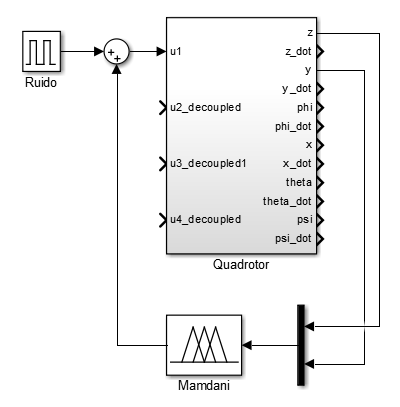
\includegraphics[width=0.5\textwidth]{./04-figuras/resultados/fis_u1/u1_mamdani_blocks}
    \label{fig:u1_mamdani_blocks}
\end{figure}

O Quadro \ref{qua:regras_fuzzy_u1_mamdani} mostra as regras definidas para o controle Fuzzy e a Figura \ref{fig:1_mamdani_surface} exibe a superfície de regras equivalente.

% Mostrar regras Fuzzy envolvidas no controle de u1 (quadro de regras + superfície)
\begin{quadro}[!htb]
    \centering
    \caption{Regras fuzzy para modelagem do controle de altitude\label{qua:regras_fuzzy_u1_mamdani}}
    \begin{tabular}{|c|c|c|}
    % \begin{tabular}{>{\centering\bfseries}m{1in} >{\centering}m{1in}
        \hline
        \textbf{{$z$}} & 
        \textbf{{$\dot{z}$}} &
        \textbf{{$u_1$}} \\
        \hline %01
            N &
            - &
            N \\
        \hline %02
            P &
            - &
            P \\
        \hline %03
            Z &
            N &
            N \\
        \hline %04
            Z &
            Z &
            Z \\
        \hline %05
            Z &
            P &
            P \\
        \hline
    \end{tabular}
    % \begin{TAB}(r,1cm,2cm)[5pt]{|c|c|}{|c|c|c|}% (rows,min,max)[tabcolsep]{columns}{rows}
    %     hi & tall one    \\
    %     hi & medium one  \\
    %     hi & standard one\\
    % \end{TAB}
\end{quadro}


\begin{figure}[!htb]
    \centering
    \caption{Superfície das regras do sistema de controle Fuzzy Mamdani para a altitude do quadrotor}
    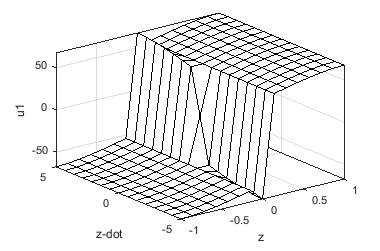
\includegraphics[width=0.6\textwidth]{./04-figuras/resultados/fis_u1/u1_mamdani_surface}
    \label{fig:1_mamdani_surface}
\end{figure}

A Figura \ref{fig:u1_mamdani_z} exibe a saída do sistema definido para controle de altitude. Como se pode ver, logo após o distúrbio, o drone alcança uma velocidade crescente negativa. Desta forma, o controlador age compensando esta velocidade para que ele possa voltar a se estabilizar na altitude que tinha inicialmente, representada por $z=0$. Como se pode ver pela Figura \ref{fig:u1_mamdani_z_regime_permanente}, a altitude $z$ nem a velocidade $\dot{z}$ voltam a ser, de fato, zero, mas ambas se aproximam bastante disso para se considerar que o drone voltou de fato à posição que assumia antes do distúrbio.

% Mostrar resultados obtidos com controle de u1
\begin{figure}[!htb]
    \centering
    \caption{Resposta das saídas $z$ e $\dot{z}$ no sistema controlado do tipo Mamdani submetido a ruído na entrada $u_1$}
    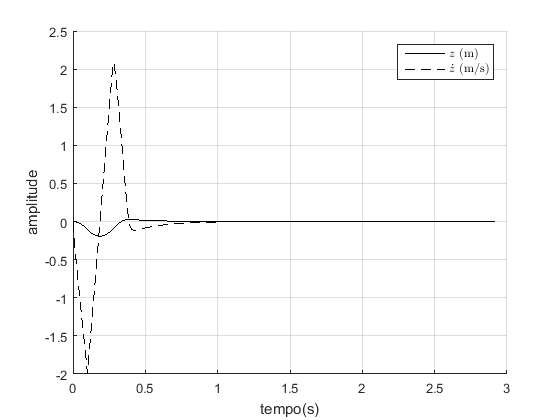
\includegraphics[width=0.8\textwidth]{./04-figuras/resultados/fis_u1/u1_mamdani_z}
    \label{fig:u1_mamdani_z}
\end{figure}

\begin{figure}[!htb]
    \centering
    \caption{Resposta das saídas $z$ e $\dot{z}$ em regime permanente do sistema controlado do tipo Mamdani para perturbação na entrada $u_1$}
    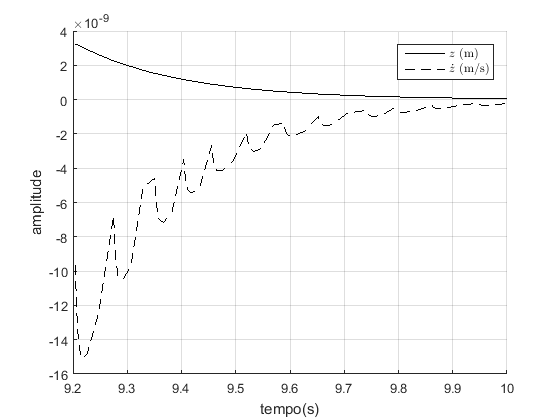
\includegraphics[width=0.8\textwidth]{./04-figuras/resultados/fis_u1/u1_mamdani_z_regime_permanente}
    \label{fig:u1_mamdani_z_regime_permanente}
\end{figure}

Assim como foi feito para o controle de atitude, para o controle de altitude também foi gerado um sistema Neuro-Fuzzy a partir do Fuzzy Mamdani originalmente criado.

Após o treinamento em processo também similar ao de controle de atitude, e mais uma vez mantendo-se as regras de origem, obteve-se a superfície de regras mostrada na Figura \ref{fig:u1_sugeno_surface}.

% Mostrar superfície Sugeno
\begin{figure}[!htb]
    \centering
    \caption{Superfície das regras do sistema de controle Fuzzy Sugeno para a altitude do quadrotor}
    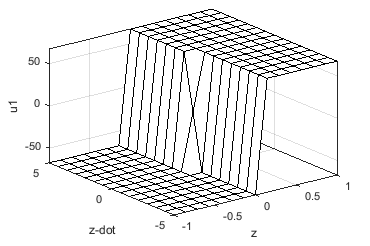
\includegraphics[width=0.6\textwidth]{./04-figuras/resultados/fis_u1/u1_sugeno_surface}
    \label{fig:u1_sugeno_surface}
\end{figure}

% Mostrar blocos com sugeno
O diagrama de blocos mostrando o sistema de controle incorporando o controlador Neuro-Fuzzy é mostrado na Figura 

\begin{figure}[!htb]
    \centering
    \caption{Diagrama do sistema de controle Fuzzy Sugeno sobre a altitude $z$}
    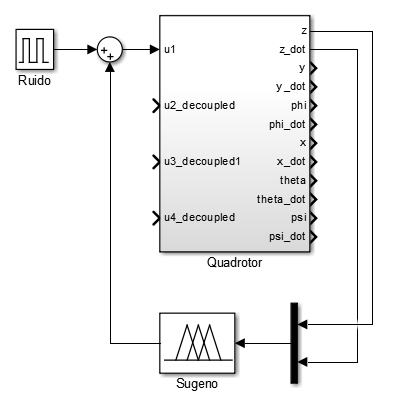
\includegraphics[width=0.5\textwidth]{./04-figuras/resultados/fis_u1/u1_sugeno_blocks}
    \label{fig:u1_sugeno_blocks}
\end{figure}

A resposta deste sistema é mostrado nas Figuras \ref{fig:u1_sugeno_z} e \ref{fig:u1_sugeno_z_regime_permanente}. Como se pode ver ao comparar as Figuras \ref{fig:u1_mamdani_z} e \ref{fig:u1_sugeno_z}, o controlador Neuro-Fuzzy reduziu a sobrelevação tanto de $z$ quanto de $\dot{z}$ além de reduzir também ligeiramente o tempo necessário para $z$ se estabilizar. Comparando as Figuras \ref{fig:u1_mamdani_z_regime_permanente} e \ref{fig:u1_sugeno_z_regime_permanente} percebe-se que o comportamento do sistema submetido aos diferentes controladores difere basante em regime permanente. No caso do controlador Mamdani, há uma variação constante de crescimento e decrescimento da velocidade $\dot{z}$. Já no caso do controlador Sugeno, as variações são menos constantes e possuem maior amplitude.

% Mostrar resultados obtidos com controle de u1
\begin{figure}[!htb]
    \centering
    \caption{Resposta das saídas $z$ e $\dot{z}$ no sistema controlado do tipo Sugeno submetido a ruído na entrada $u_1$}
    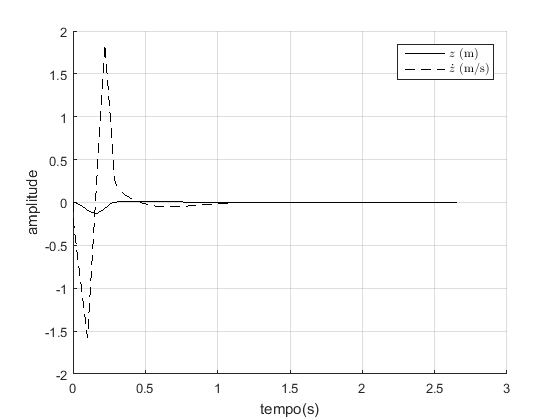
\includegraphics[width=0.8\textwidth]{./04-figuras/resultados/fis_u1/u1_sugeno_z}
    \label{fig:u1_sugeno_z}
\end{figure}

\begin{figure}[!htb]
    \centering
    \caption{Resposta das saídas $z$ e $\dot{z}$ em regime permanente no sistema controlado do tipo Sugeno submetido a ruído na entrada $u_1$}
    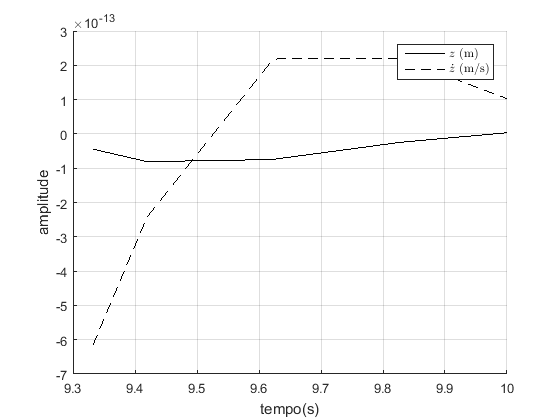
\includegraphics[width=0.8\textwidth]{./04-figuras/resultados/fis_u1/u1_sugeno_z_regime_permanente}
    \label{fig:u1_sugeno_z_regime_permanente}
\end{figure}



